%% 
%% Copyright 2007-2020 Elsevier Ltd
%% 
%% This file is part of the 'Elsarticle Bundle'.
%% ---------------------------------------------
%% 
%% It may be distributed under the conditions of the LaTeX Project Public
%% License, either version 1.2 of this license or (at your option) any
%% later version.  The latest version of this license is in
%%    http://www.latex-project.org/lppl.txt
%% and version 1.2 or later is part of all distributions of LaTeX
%% version 1999/12/01 or later.
%% 
%% The list of all files belonging to the 'Elsarticle Bundle' is
%% given in the file `manifest.txt'.
%% 
%% Template article for Elsevier's document class `elsarticle'
%% with harvard style bibliographic references

\documentclass[final,times,twocolumn,article]{elsarticle}

%% For including figures, graphicx.sty has been loaded in
%% elsarticle.cls. If you prefer to use the old commands
%% please give \usepackage{epsfig}

%% The amssymb package provides various useful mathematical symbols
\usepackage{amssymb}
\usepackage{lipsum}

%% The amsthm package provides extended theorem environments
%% \usepackage{amsthm}

%% The lineno packages adds line numbers. Start line numbering with
%% \begin{linenumbers}, end it with \end{linenumbers}. Or switch it on
%% for the whole article with \linenumbers.
%% \usepackage{lineno}

%% You might want to define your own abbreviated commands for common used terms, e.g.:
\newcommand{\kms}{km\,s$^{-1}$}
\newcommand{\msun}{$M_\odot}

\journal{Astronomy $\&$ Computing}


\begin{document}

\begin{frontmatter}

%% Title, authors and addresses

%% use the tnoteref command within \title for footnotes;
%% use the tnotetext command for theassociated footnote;
%% use the fnref command within \author or \affiliation for footnotes;
%% use the fntext command for theassociated footnote;
%% use the corref command within \author for corresponding author footnotes;
%% use the cortext command for theassociated footnote;
%% use the ead command for the email address,
%% and the form \ead[url] for the home page:
%% \title{Title\tnoteref{label1}}
%% \tnotetext[label1]{}
%% \author{Name\corref{cor1}\fnref{label2}}
%% \ead{email address}
%% \ead[url]{home page}
%% \fntext[label2]{}
%% \cortext[cor1]{}
%% \affiliation{organization={},
%%            addressline={}, 
%%            city={},
%%            postcode={}, 
%%            state={},
%%            country={}}
%% \fntext[label3]{}

\title{Discovering cysteine protease covalent inhibitors using deep learning message passing networks}

%% use optional labels to link authors explicitly to addresses:
%% \author[label1,label2]{}
%% \affiliation[label1]{organization={},
%%             addressline={},
%%             city={},
%%             postcode={},
%%             state={},
%%             country={}}
%%
%% \affiliation[label2]{organization={},
%%             addressline={},
%%             city={},
%%             postcode={},
%%             state={},
%%             country={}}

\author[first]{Carla Feliu}
\affiliation[first]{organization={University of Vic - Central University of Catalonia},%Department and Organization 
            city={Vic}}

\begin{abstract}
%% Text of abstract
Example abstract for the astronomy and computing journal. Here you provide a brief summary of the research and the results. RESUM DE TOT
\end{abstract}

%%Graphical abstract
%\begin{graphicalabstract}
%\includegraphics{grabs}
%\end{graphicalabstract}

%%Research highlights
%\begin{highlights}
%\item Research highlight 1
%\item Research highlight 2
%\end{highlights}

\begin{keyword}
%% keywords here, in the form: keyword \sep keyword, up to a maximum of 6 keywords
keyword 1 \sep keyword 2 \sep keyword 3 \sep keyword 4

%% PACS codes here, in the form: \PACS code \sep code

%% MSC codes here, in the form: \MSC code \sep code
%% or \MSC[2008] code \sep code (2000 is the default)

\end{keyword}


\end{frontmatter}

%\tableofcontents

%% \linenumbers

%% main text

\section{Introduction}
\label{introduction}

Proteases, also known as peptid hydrolases, are enzymes capable of catalysing hydrolytic reactions that degrade protein molecules to peptides, and finally to free amino acids. They also carry out proteolytic reactions, and regulate various enzymatic cascades that form part of metabolic cycles. \cite{Ramos2019} The role they play is key in carrying out vital biological processes, such as the regulation of various cellular processes as well as differentiation, gene expression and cell death. Protests are a very broad group of enzymes that are differentiated by, among other things, the type of amino acid residue in their catalytic site. \cite{Ramos2019}

Cystein proteases (also known as thiol proteases), are one of the types of proteases that exist, and are characterised by catalysing the breakdown of proteins by cleavage of peptide bonds using a cysteine nucleophile tilo. These proteases are classified into two types according to their location within the organism; Catepsins, located in the lysosome, and Calpains, located in the cytosol. \cite{Gupta2020}

Although these proteases have a key role in vital processes, when there is overexposure or dysregulation in pathological conditions, they can contribute to the development of many diseases.  In several studies, it has been shown that cathepsins, located in the lysosome, are related to tumour progression. \cite{Berdowska2004} \cite{Mohamed2006}. These cystein proteases allow cancer cells to attack nearby tissues, blood and lymphatic vessels and metastasise to peripheral tissues. \cite{Gupta2020} \cite{Gocheva2006} For this reason, the search for inhibitors of cystein proteases has become an objective in medical and pharmacological research, in order to develop new therapeutic opportunities. \cite{cath}

The interest of cystein proteases as targets is related to the fact that by working with their inhibition, it is possible to find therapies for many of the diseases they are involved in. They are also interesting targets due to the reactive cisterna active site, as the high nucleophilicity of the cisterna thiol, under physiological conditions, provides an ideal anchoring site for small electrophilic molecules. \cite{Maurais2019} 

The inhibition process is defined by the effectiveness of the binding of a protein to the selected targets. This depends on the reaction equilibrium between the functional groups of the drug and the active site residues of the protein. This balance is determined by the type of interaction that is created, and can be either covalent or non-covalent interactions. 
Covalent bonds are usually formed by the interaction of certain amino acids, including the nucleophilic cisterna and a reactive functional group of the ligand. They are more effective due to their long permanence in the active site, high binding affinity and high selectivity and specificity, resulting in complete inhibition of the target compared to the reversible effect of non-covalent drugs. \cite{Aljoundi2020} 

The drug development process is a very elaborate process, which can involve a lot of time and resources. It begins with the search for and characterisation of a possible biological target for a specific disease or enzyme, and then the process of creating the most suitable therapeutic compound begins. Before reaching drug development, many molecular properties must be optimised to identify and validate the target, as this is one of the most important steps in drug development. \cite{Hughes2011}
Historically, this search was guided by the calculations and intuition of expert scientists, but with the great advances in new technologies and the increase in resources, it has been possible to apply new methods that are much faster and more reliable. \cite{Hop2018}

One of the most used methods currently for this drug development, and which has allowed a great advance in this field of medical research, making the process less expensive and more efficient, is machine learning (ML). ML is a branch of artificial intelligence (AI) that applies computer algorithms with the ability to learn themselves from dirty, raw data, to then perform a specific task. Within ML methods, the most widely used and expanding is deep learning (DL). It is inspired by the information processing patterns of the human brain and is designed using multiple layers of algorithms (artificial neural networks, ANNs), each of which makes an interpretation of the data it has received. \cite{Alzubaidi2021} 

Artificial neural networks, are created to simulate a network of model neurons on a computer. By applying algorithms that mimic the processes of real neurons, models are generated that learn to solve many types of problems. The networks are composed of artificial neuron units, capable of transmitting signals to each other.(what are artificial networks ). Each reception of a signal in the neurons is associated with a weight that varies as learning progresses, which can increase or decrease the strength of the signal that will then be sent to the other neurons. These signals pass the multilayers of artificial neurons until they reach the final layer, where the result of these connections is the prediction of the algorithm. \cite{Talevi2020}

The chemprop Architecture is a neural network built for the prediction of molecular properties that includes a directed message passing neural network (D-MPNN) module for molecular feature extraction and a feed-forward neural network (FNN) for property prediction. This model takes molecular SMILES as input and extracts all the atomic and bonding characteristics of the molecules to generate a single vector of characteristics which, by entering it into the FNN, can predict the activity of the candidate molecules. \cite{Wang2022}

Given the growing interest in cysteine proteases as targets for therapeutic treatments and the availabikity of new machine learning tools for these drug discovery processes, three questions are raised in this work.

\begin{itemize}
    \item Is it possible to identify covalent targets that can serve as inhibitors for cysteine proteases using ANN?
    \item What is the best way to train a model using ANN?
    \item Is it possible to identify molecular patterns or specific molecules that can help us in finding cysteine protease inhibitors in two completely different databases?
    
\end{itemize}

%%\section{Objectives}

We will use a ML model, ANN, applying a known dataset of compounds that interact with cysteine proteases. This dataset will be used to train our model, allowing us to make predictions from two different databases, that lead us to solve the proposed questions.

Specific objectives:

\begin{enumerate}
    \item Identify a database with known targets of cysteine proteases that includes inhibitory activity, which will serve as the training data of our ML model. 
    \item Download the database and extract the (Simplified Molecular Input Line Entry Sistem)SMILES information. Prepare the required dataframe structure for working with the ML algorithm, obtaining various features for each molecule and its inhibitory activity (IC50).
    \item Train the chemprop model using various approaches, evaluating which one makes the model more stable for our predictions. 
    \item Identify suitable databases to obtain the molecules for our predictions. Similar to the training dataframe, construct the structure necessary to make the predictions with our training model. 
    \item Analyze the data generated from the predictions made by the ML model, checking the correlation of the data and their similarity to understand if the predictions obtained are suitable for our questions raised. 
    \item Detect patterns of molecules that could be optimal for working in the discovery of cystein protease inhibitors. 
\end{enumerate}

\section{\textbf{Methods}}

\subsection{Machine learning model}

To carry out the study and work with the Machine Learning algorithm, we have used the the Visual Studio Code editor to generate all the necessary code in the python programming lenguage. 

Machine Learning is an expansive field where various algorithms and models can be used to achieve multiple objectives. In this study, we developed code that uses a deep learning model incorporating a directed message passing neural network (D-MPNN) to obtain predictions. 

We employed the Chemprop architecture, an open-source machine learning framework. This framework includes a D-MPNN module for molecular feature extraction and a feed-forward neural network (FNN) for property prediction. To work with this algorithm, input in SMILES format (representing chemical formulas) is required. The algorithm then transforms this input into a molecular graph structure, where atoms serve as nodes, and bonds as edges. 

The D-MPNN module plays a crucial role in extracting specific features for all the atoms, creating a dataset that represents the entire molecule. Information flows unidirectionally from the input layer to the final output layer. Then, the resulting vector is employed in the FNN module for making predictions regarding the activity of the molecules studied. \cite{Wang2022}

A deep learning artificial neural network can solve classification or regression problems. Classification problems involve the use of labels, where data must be categorized into multiple categories. On the other hand, regression problems require the specification of a numerical quantity to classify variables. In this work, we have focused on regression problems, using the IC50 value variable extracted from the ChEMBL database, which classifies molecules on their interaction activity. 

\subsection{Datasets}

In this study, we worked with three different databases to extract the necessary information for our research. Data extraction has been performed depending on each database.  

\subsubsection{ChEMBL}

ChEMBL is a database of bioactive small molecules similar to drugs, containing calculated properties and bioactivities. \cite{chemblweb}

Our interest in this database is to obtain information about molecules that can interact with cysteine proteases in order to establish a reference point for interaction activity, allowing us to train our ML model. To access the relevant information to our study, we filtered the ChEMBL database with the term "cysteine protease" and extract the resulting targets. Once we obtained the cysteine protease targets, we used the python "requests" module to retrieve information about all the molecules interacting with each of the targets, along with their interaction activity, represented by the -log(IC50 molar) value. The value was used to train our ML model. 

\subsubsection{ChemDiv}

ChemDiv is a globally recognized research organization in drug discovery solutions. They have identified specific libraries aimed at addressing varius targets, protein domains, cellular processes and more. \cite{chemdivweb}

From this database, we obtained the "Cysteine Targeted Covalent Library", which consists of 39,301 compounts with specific warheads designed to react with cysteine. The objective of using this library is, by applying our trained model, to find possible compounds that exhibit significant interaction activity with cysteine. This will help us identify patterns that can be used to understand what type of molecule could be a good inhibitor. 

\subsubsection{Zinc}

ZINC

\subsection{Data preparation and curation}

To carry out the process of training machine learning models effectively, it is crucial to have suitable and properly prepared dataset. Therefore, prior preparation is required. 

This data structure should have a first column containing the SMILES of the molecules, features describing the molecules, and finally, in a last row, the interaction activity of these molecules, the IC50 value. Data preparation also includes conducting a thorough analysis of the data structure, which is essential for a deep understanding of the data and, consequently, for conducting a more accurate result analysis. 

\subsubsection{Train}

To prepare the training data, we started with a list of all the targets that interact with cysteine proteases and their interactions, from the ChEMBL database. These initial data will provide us a lot of information, but there is an important data preprocessing step before introducing the dataframe into our model. 

From this dataframe containing the intereactions of the cystein proteasa targets, we extracted the list of all the ChEMBL IDs of the molecules that interact with them, along with their IC50 activity values. Using a ChEMBL API and Python function, we obtained the SMILES for each of the registered molecules. 

The data cleaning process is very important, which includes the removal of null values, as they represent a lack of information that may not be accepted or could influence the outcome of the algorithm, and the elimination of duplicated SMILES to avoid duplicated information. 

To prepare the training data, we used the chemoinformatics and machine learning software RDKit\cite{rdkit}. From this software, we employed a Python function to iterate over each SMILE, resulting in a total of 10 different features extracted from each compound. 
In order to ensure and assess the quality of the trained model, we conducted four trainings using four slightly different feature dataframes. These dataframes were analyzed, and ultimately, we determined which one is the most suitable for analyzind our data. 

\begin{itemize}
\item Train 1: No curated and no normalized data.
\item Train 2: Curated and no normalized data.
\item Train 3: Curated and z-score normalized data.
\item Train 4: Curated and MinMaxScaler normalized data.
\end{itemize}
\subsubsection{Predict}

The first prediction was carried out using data from ChemDiv. To extract this data, we specifically selected the ChemDiv Cysteine Targeted Covalent Library to obtain the initial results. 

We downloaded the database using a Python function that uses the "requests" package to access the URL of the corresponding ChemDiv library. This returned an SDF file with all the information for each molecule. Using a function that accesses the previously mentioned RDKit module, we created a dataframe composed of the first column with SMILES, followed by 10 different features for each molecule. In this case, we didnt' include the IC50 activity, as this will be obtained from the ML model. 
To prepare the data for inpot into the algorithm, we performed a curation similar to the one mentioned in the training data preparation. Additionally, we added 200 molecules extracted from the dataframe used to train the model, as these molecules have been entered into the system with real and validated values, providing a reference. Finally, to ensure that the data have the same distribution to the trained model that will be used, we performed a MinMaxScaler normalization. 

The second prediction was carried out with data from the general Zinc database, obtaining only a portion to work with a more manegeable data quantity. It was used to address the goal of finding patterns within a general database, without especificity to cysteine proteases. 

From Zinc, we downloaded a .uri file that contains the total database distributed across diferents URLs. Using Python's wget control, we accessed all of these URLs and downloaded the data, resulting in multiple files that collectively comprise the Zinc database. Subsequently, using a python function, we downloaded three of these files, each containing a multitude of molecules. The resulting dataframe from this download consists fo SMILES along with corresponding ZINC IDs. 

Through a function that uses RDKit, we filtered out invalid SMILES to minimize potential errors before preparing the dataframe for the algorithm. Similarly to what we mentioned earlier for the other dataframes, we used a function with RDKit to generate the appropriate matrix for inputting into the algorithm, with the first column containing the SMILES, followed by 10 features for each one. 

Finally, as we did with the first dataframe prediction, we added the same 200 molecules extracted from the training dataframe and normalized data with MinMaxScaler. 

\subsection{Results data analysis}

Once the result of the prediction from the used model was obtained, an analysis was conducted to assess the residual error of the resulting prediction. The 200 reference molecules, which were used both for training and obtaining the predictions, were used to generate a histogram and a regression line. This analysis allows us to visualize the model's error and the reliability of our data. 

To analyze and draw conclusions from the results, correlation graphs of the variables were generated for the two predictions made, in order to observe the relationship between all the calculated features. Additionally, a correlation graph of all the features with the IC50 activity value calculated by the model was created. 

Finally, based on the results of the two predictions from the different databases, a selection of the molecules with a higher -log(IC50 molar) value was made, generating a dataframe for each prediction of the 10 molecules showed stronger interactions. To conclude, a similarity analysis was conducted. This will enable us to observe and analyze if there is a pattern among the molecules with higher activity, providing an indication of whether our model aligns with the objective or not. 

\section{Results}
%%\label{Results}

The different dataframes prepared for training the model, originated from a dataset with 19,262 molecules. In the case of train 1, a less elaborate data curation was performed, resulting in a dataframe with 19,172 molecules. For the train 2, starting from the same database, a more elaborated data curation was carried out, eliminating duplicated SMILES, reducing the number of molecules to 11,703. Train 3 and Train 4 were prepared by the dataset from Train 2 and normalizing the data using z-score and MinMaxScaler, respectively. (Table~\ref{Table1})

\begin{table}[ht]
\centering
\begin{tabular}{l c c c} 
     \hline
     Train & Initial dim. & Data curated & Norm.\\ 
     \hline
     Train 1 & 19,262 & 19,172 & No\\
     \hline
     Train 2 & 19,262 & 11,703 & No \\
     \hline
     Train 3 & 19,262 & 11,703 & Z-Score\\ 
     \hline
     Train 4 & 19,262 & 11,703 & MinMaxScale\\ 
     \hline
    \end{tabular}
\caption{Training sets}
\label{Table1}
\end{table}

In both Table~\ref{Figure1} and Figures~\ref{Figure2} and ~\ref{Figure3}, the evaluation metrics of the training models are presented, where we can see the different results: 

\begin{itemize}
\item Mean Absolute Error (MAE): MAE is a measure of the average difference between the model's predictions and the actual values. The closer MAE is to 0, the better the model's performance, as it indicates that the predictions are closer to the actual values. As can be seen in the results of the mentioned figures, training model 4 shows the best performance in this aspect, while training model 1 performs the worst.
\item Mean Squared Error (MSE): MSE takes the square of the differences between predictions and actual values and calculates an average. The lower the value, the better the model's performance. In the mentioned figures, it can be observed that training model 4 continues to have the best performance, while training model 1 performs the worst.
\item Coefficient of Determination (R2): It is a measure that assesses how well the predictions fit the actual values. This value varies from 0 to 1, where 1 indicates a perfect fit to the model, and 0 indicates no fit at all. In this result, we see that the model that approaches 1 the closest and therefore fits better is training model 2, followed by training models 4 and 3, which have the same R2 value with very little difference from 2. Finally, training model 1 is the furthest from a perfect fit.
\item Root Mean Squared Error (RMSE): RMSE is the square root of MSE and is used to provide an average of the model's error. The lower it is, the better the model's performance. In this result, training model 1 stands out by a significant margin as having the best performance.
\end{itemize}

The results obtained from the 4 training runs conducted with the ML model algorithm show that the model with the highest possibility of error is training model 1, prepared with less elaborate data curation and with non-normalized data, while the one with the most reliable prediction is training model 4, with stricter data curation and a MinMaxScaler normalization. With the training results analysis, it is decided to use Train 4 to obtain the predictions for our study. 

\begin{figure}[ht]
    \centering 
     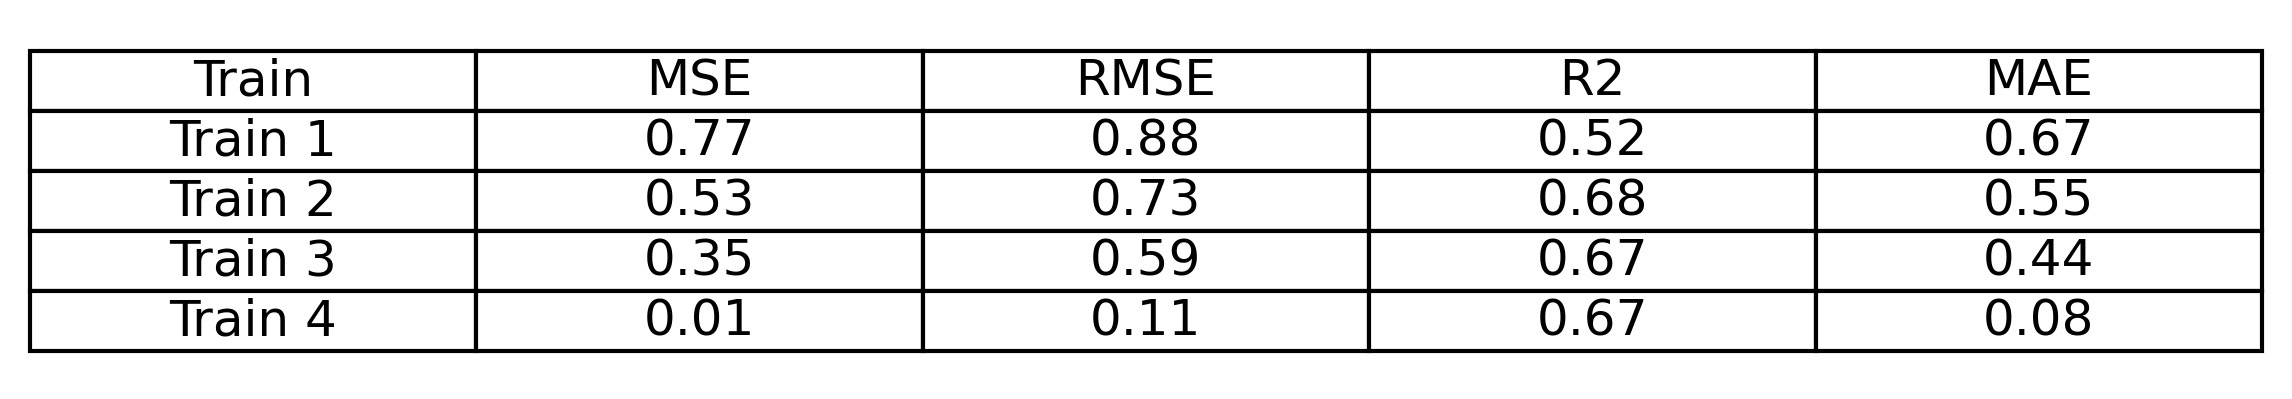
\includegraphics[width=0.4\textwidth]{/Users/carlafeliu/Docs/Master/TFM/github/TFM/output/results_train.jpeg}	
     \caption{Training set results metrics} 
     \label{Figure1}
 \end{figure}
 
 \begin{figure}[ht]
     \centering 
      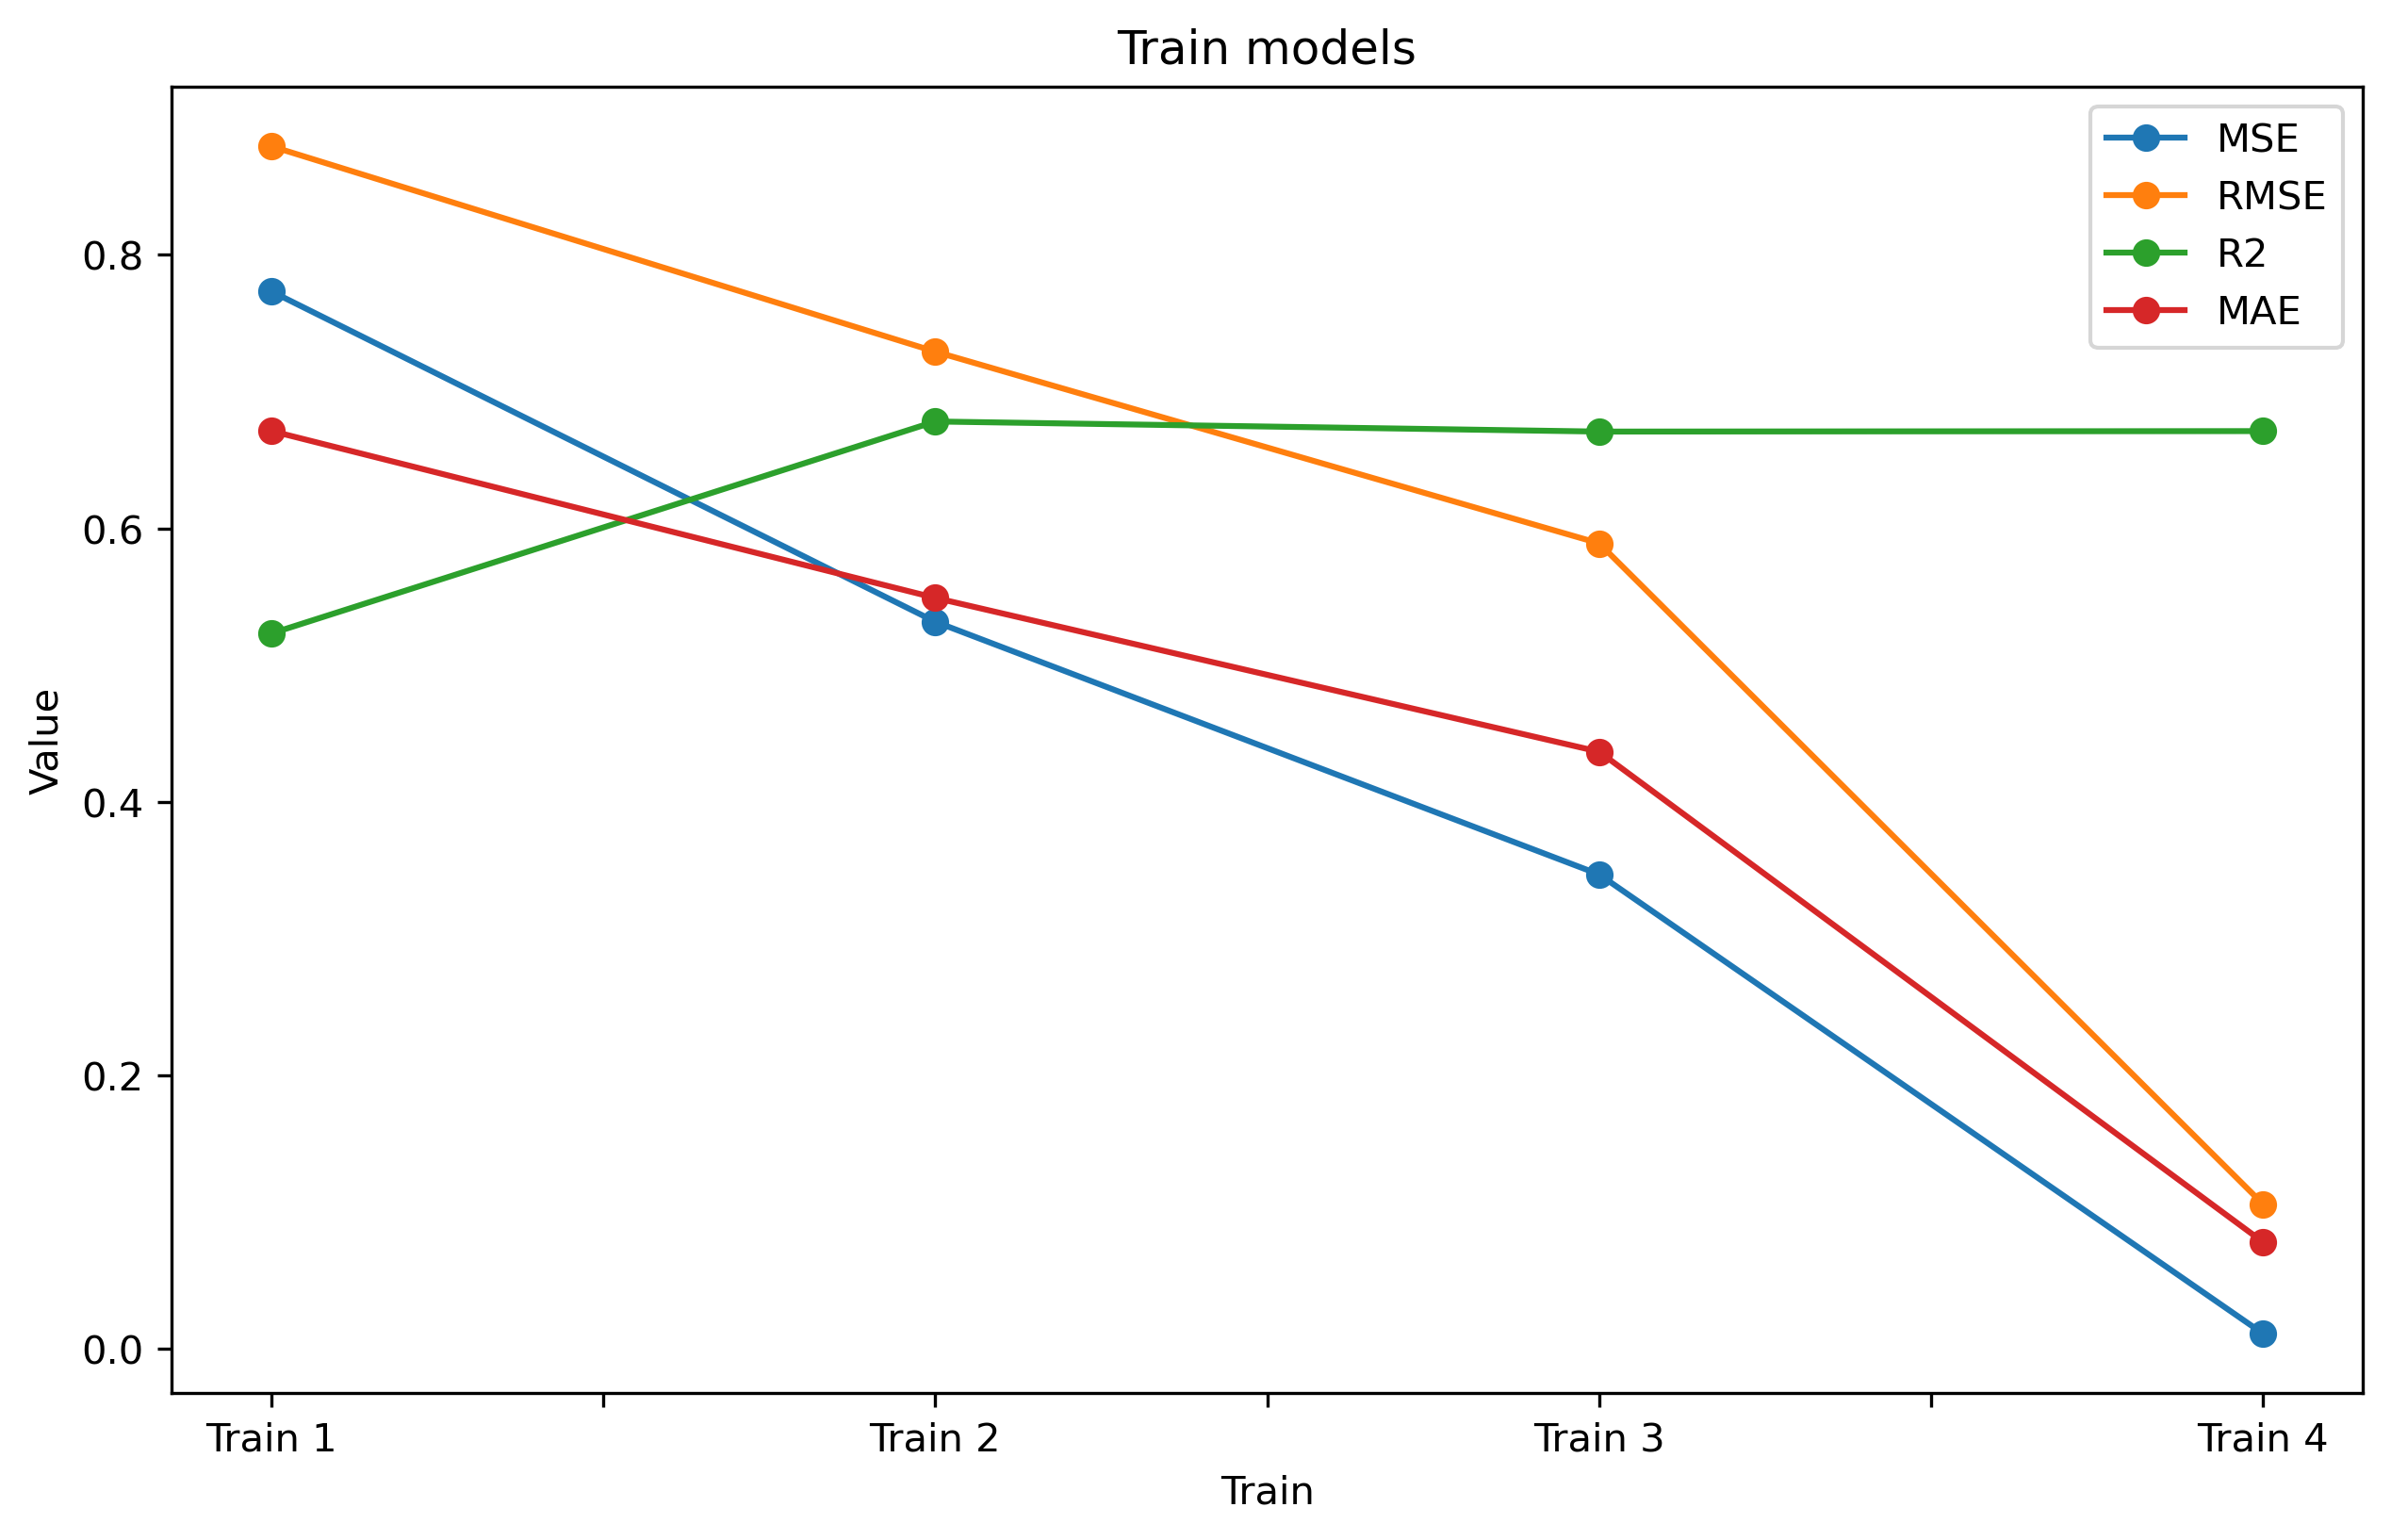
\includegraphics[width=0.4\textwidth]{/Users/carlafeliu/Docs/Master/TFM/github/TFM/output/plot_results_train.png}	
      \caption{Line chart of training set results metrics} 
      \label{Figure2}
  \end{figure}
 
  \begin{figure}[ht]
     \centering 
      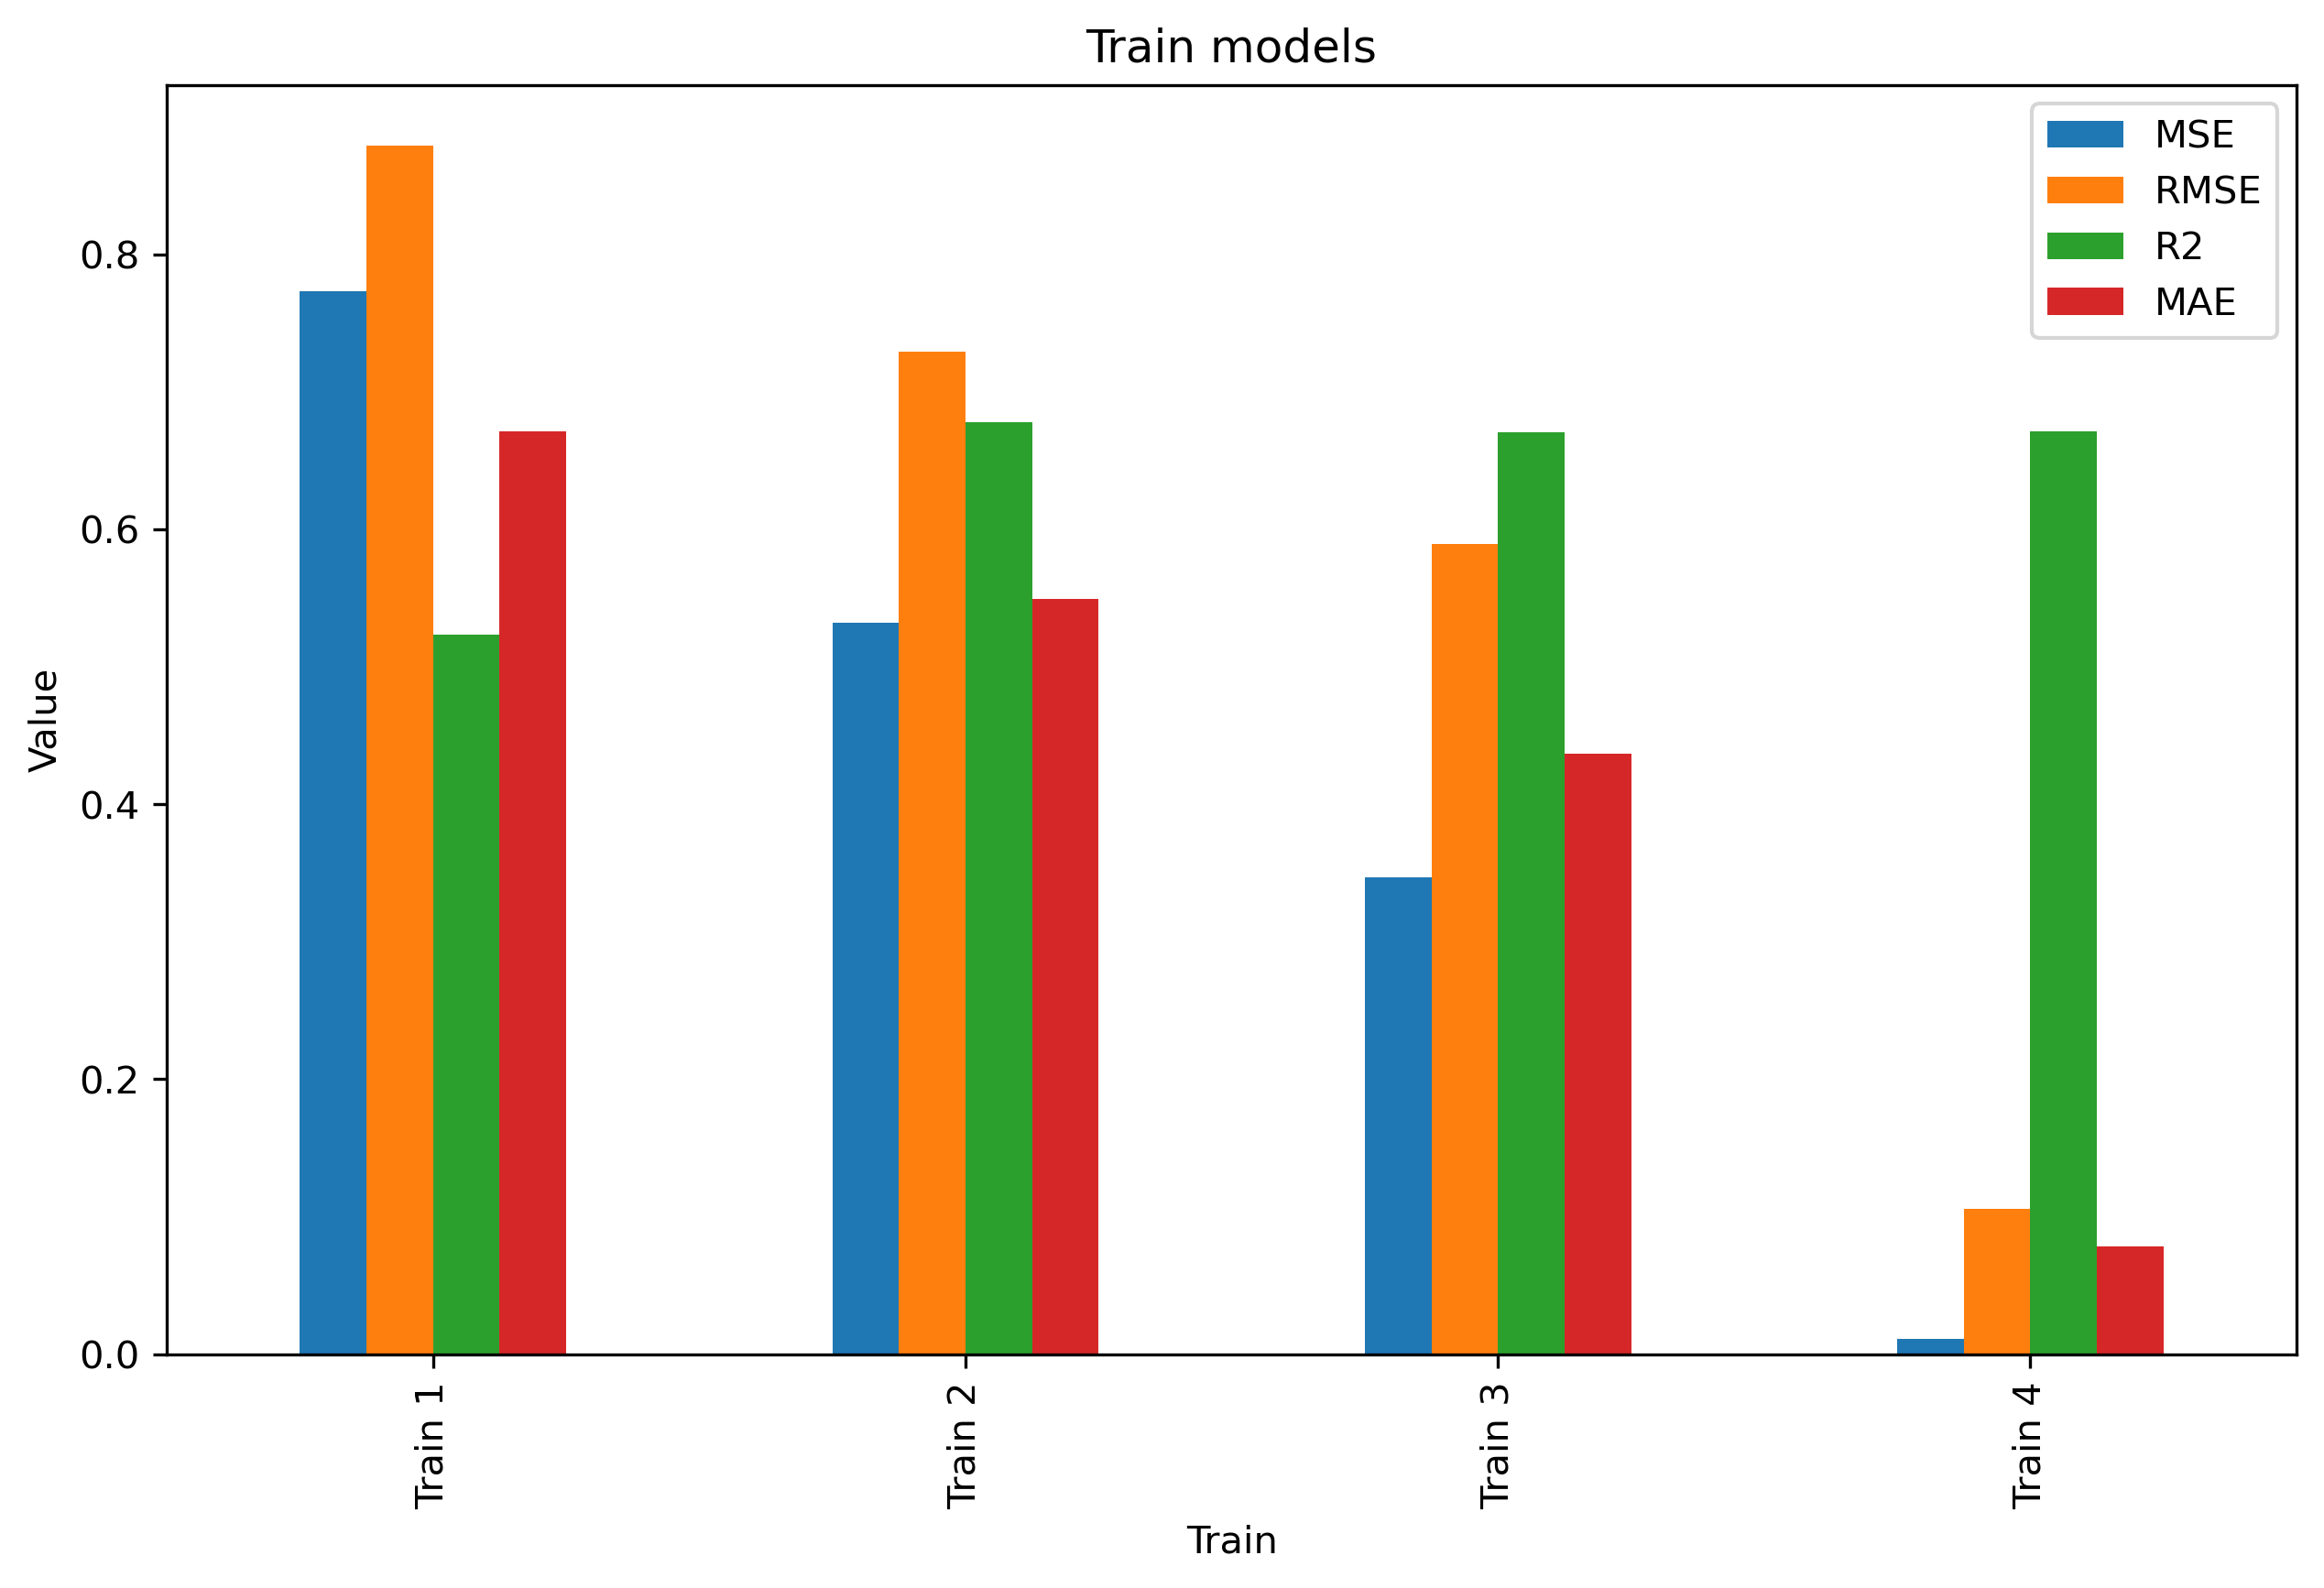
\includegraphics[width=0.4\textwidth]{/Users/carlafeliu/Docs/Master/TFM/github/TFM/output/bar_results_train.png}	
      \caption{Barplot of training set results metrics} 
      \label{Figure3}
  \end{figure}

Once the model predictions have been made, the results of the 200 molecules used for training, for which we already had information about inhibitory activity, were compared with the same 200 molecules resulting from the prediction. In the case of these ones, the algorithm generates a prediction of the activity because when inputting the dataset into the model for prediction, this information was not included. 

Whan analyzinc the results of the histogram (Figure~\ref{Figure4}), it is noted that the distribution of the data is not perfect. Although the figure could suggest a pattern that indicate a good distribution, there are many intermediate values that generate multiple peaks that don't follow the same trend. This can also be observed with the regression line (Figure~\ref{Figure5}), which does not fit the central line of the actual values, indicating that it does not fully adapt to the real values. Furthermore, it can be observed how this dispersion in the distribution increases with higher values. 

\begin{figure}[ht]
    \centering 
     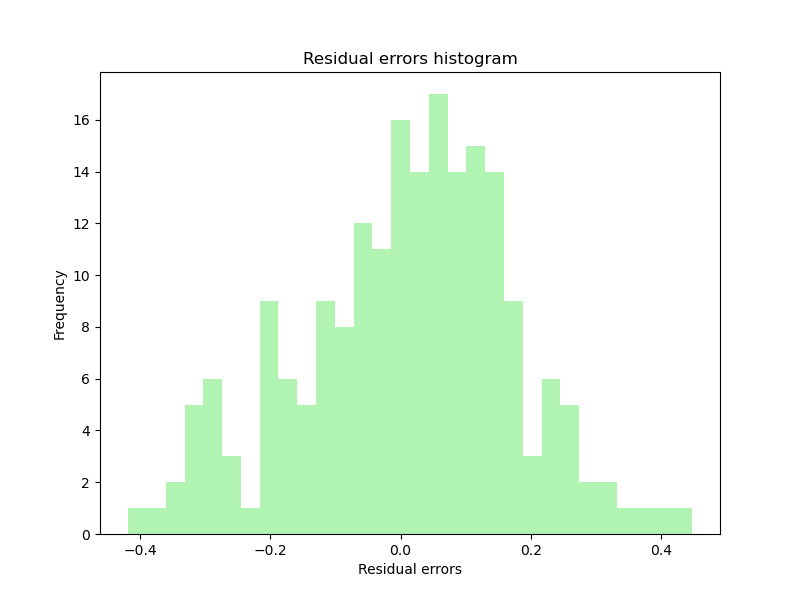
\includegraphics[width=0.4\textwidth]{/Users/carlafeliu/Docs/Master/TFM/github/TFM/output/residual_error_predict_chemdiv.png}	
     \caption{Histogram of predicted residual errors} 
     \label{Figure4}
 \end{figure}

 \begin{figure}[ht]
    \centering 
     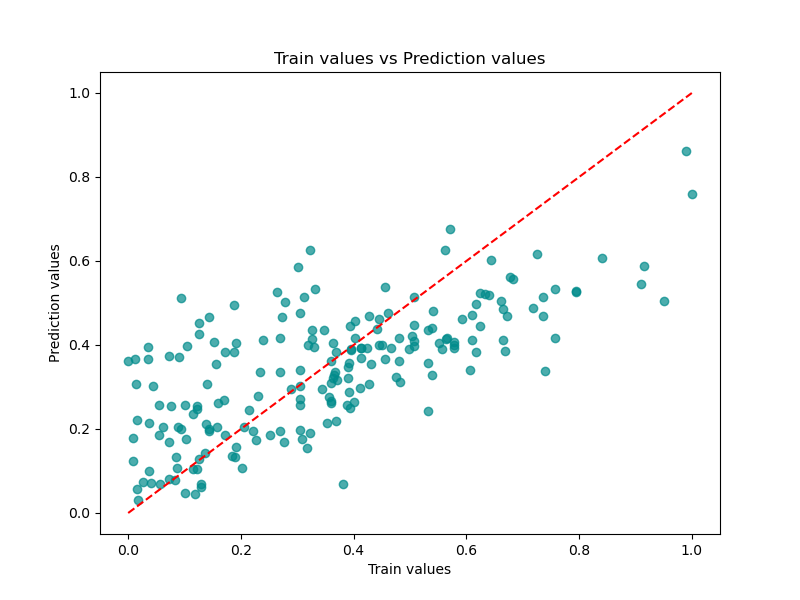
\includegraphics[width=0.4\textwidth]{/Users/carlafeliu/Docs/Master/TFM/github/TFM/output/linregresion_predict_chemdiv.png}	
     \caption{Linear regression of predicted residual errors} 
     \label{Figure5}
 \end{figure}




\section{Discussion}
%%\label{}


\section{Conclusions}


\section*{Acknowledgements}
Thanks to ...

%% The Appendices part is started with the command \appendix;
%% appendix sections are then done as normal sections
\appendix

\section{Appendix title 1}
%% \label{}

\section{Appendix title 2}
%% \label{}

%% If you have bibdatabase file and want bibtex to generate the
%% bibitems, please use
%%

\section{Bibliography}
\bibliographystyle{unsrtnat} 
\bibliography{library}



\end{document}

\endinput
%%
%% End of file `elsarticle-template-harv.tex'.
